\chapter{Background \& Related Work}
\section{Background}
In this section, I will list all technologies that are used in this project along with discussing other papers which were trying to address security with IoT devices by also trying to include blockchain technology.
\subsection{MQTT}
When designing architecture with the main target being communication of many (even couple of thousands a second) clients constantly exchanging data, scalability and availability needs to be kept in mind. The first and obvious solution would be to directly connect data consumers and data produces, by making them communicate in Peer-to-Peer fashion, removing the need for any extra infrastructure. This might work perfectly fine with small systems (disregarding issues such as dynamic DNS or static IP), but as number of clients requesting access to data increases, the total capacity of the sensor would eventually be capped - since IoT usually are of limited power and computation capacity. Imagine a scenario where a single temperature sensor constantly getting bombarded with requests for current readings, it might be able to cope up to 5 incoming requests every second, everything else would cause malfunction or significantly slower response times.

Then there is also an issue of security. By allowing clients to connect to our IoT devices, we are opening an extra attack vector. What if the client doesn't want to only access the temperature readings, but perhaps inject a worm which would intercept other sensors (such as cameras). Recently ``smart nannies'', responsible for alerting the parents when the child is crying and also relieving the adults from having to be constantly nearby, gained popularity. A direct camera feed could be accesses via smart phone, no matter where. This eventually led to exploitation, as it was found that many of those devices were vulnerable to remote access by third parties\cite{pultarova2016webcam}.

MQTT aims to address those issues (and not only), by moving the communication to a separate entity, which operates in a publish-subscribe fashion. This would mean that IoT devices only have to publish information that is available to them (e.g. temperature readings), allowing to completely remove remote access, effectively mitigating this particular attack vector. Furthermore, the MQTT brokers can be further placed behind load balancers and such to further enhance their availability.

\begin{figure}[ht]
    \centering
    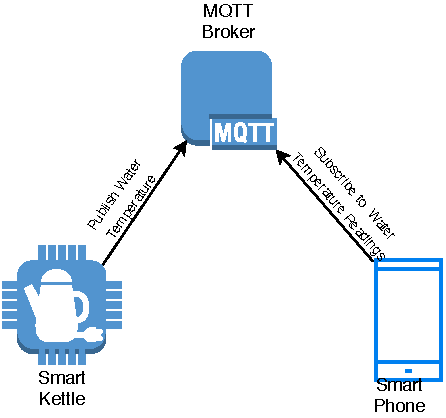
\includegraphics[width=0.5\textwidth]{mqtt_demo}
    \caption{MQTT Broker Architecture}
    \label{fig:mqtt}
\end{figure}

In short, MQTT, fully expanded to Message Queueing Telemetry Transport is an open protocol, certified by OASIS and ISO\cite{banks2019mqtt}, responsible for publisher-subscriber architecture. It's important to point out that MQTT is not a piece of software or a server, but rather a set of standards defining what potential clients can expect (what kind of responses and data) while connection to brokers following the standard. Figure \ref{fig:mqtt} briefly shows how MQTT-compatible broker can relay information between clients. Smart Phone and Smart Kettle don't have to be online at the same time in order to receive information, nor Smart Phone is even permitted to initiate direct connection to Smart Kettle. The broker's responsibility is to track connected subscribers (which must specify topic of their interest) and maintain connection until subscribe advertises session termination or abruptly disconnects (e.g. loss of power or unreliable connection).

In MQTT architecture, Client ID identifies each of the connecting entities (publisher / subscriber) and Topic identifies a bridge between publishers and subscribers connected to the same topic. For example, a Smart Kettle could be publishing temperature readings under topic called ``UK/Aberdeen/Kettle'' - then, Smart Phone would need to request the same topic to receive those readings. 

\subsubsection{\textbf{Message persistence}}
This will be discussed in depth, when I will describe the process of publishing and subscribing, but it's worth pointing out that by default, the messages are not saved nor cached on the broker. That is, if Kettle publishes the temperature reading, but there is no subscribers listening to this information, the message will perish. This is not ideal, for situation where smart device could wake up only every couple of minutes and then go to low-power mode again. To address this, MQTT Messages can be enriched by ``Retain'' flag. If such flag is present, the broker will keep the message and send it straight away to any new subscribers requesting given topic. This is also useful for issuing commands to IoT devices - for example, a phone could send command to turn off the lights with ``Retain'' flag set. Then, the smart light switch could check for retained messages every couple of minutes, removing the need of constant connection.

\subsubsection{\textbf{Implementation}}
MQTT by itself is only a collection of standards instructing implementors on what patterns should be followed and the structure of particular messages, thus it's not shipped with any piece of software. It assumes operation on TCP layer of network (although newer versions also allow for WebSocket support \citep{mijovic2016comparing}), thus also allowing for encrypted connection via Transport Layer Security. Every exchanged message is a TCP packet, following strict convection - which in case of deviation is discarded as corrupted.

Two of the implementations that I have considered during this project are Mosquitto\footnote{https://mosquitto.org/} by Eclipse and Moquette\footnote{https://github.com/moquette-io/moquette}. The former written in C and the former in Java, although there is many, many more. In a paper by \citet{de2019performance}, scientists compare Moquitto and RabbitMQ, arguining their choice by the offered cloud infrastructure with greater scalability opportunities. Moreover, there are solutions that are paid, whereas the considered approaches are free and open source allowing for better understanding of operations. The paper is concluded with the finding that hardware and network latency has a far greater impact on the performance, rather than choice of the individual broker, which leaves the decision mostly down to offered extra features.

Mosquitto also offers a Docker container \cite{light2017mosquitto} in which the broker can be run, allowing for further isolation and removal of extra dependencies.

\subsubsection{\textbf{Publishing}}

The most popular method of passing MQTT messages is still under Transport layer, as TCP packets. This allows for slightly higher freedom (compared to stricter protocols, such as HTTP), at the cost of more sophisticated parsing. MQTT standard is composed of several message types with the most important being:
\begin{itemize}
  \item CONNECT - used to initiate the connection
  \item PUBLISH - used by the client to publish messages and by the broker to publish messages to subscribers
  \item SUBSCRIBE - used by the client to request subscription to a given topic
  \item UNSUBSCRIBE - used by the client to request removal of subscription to given topics
  \item Along with relevant *ACK counterparts (e.g. CONNACK) used to indicate successful transmission of the message
\end{itemize}
As shown on figure \ref{fig:mqtt_publish}, the publishing flow starts with the CONNECT messages. Inside, there are several flags included, such as Quality of Service requested (MQTT can periodically send heartbeat ping to clients to check if they are still alive), requested version of MQTT protocol (at the moment, v5.0 and v3.1). This part is also referred as ``Variable header''. The second part, known as ``Payload'' consists of client ID.

Then, once the client has established its identity to the broker, the broker responds with CONNACK message, which contains bit informing whether further connection is allowed or not. From this point, the client is cleared to start publishing session.

Usually, for every message to be published, there is one PUBLISH packet. Newer version of MQTT allow for spreading larger messages across multiple packets, although this will not be covered in this paper. The PUBLISH packet contains mostly two properties - topic to be published on and the actual payload. Each of the properties is prepended with 8 bytes indicating the length. From this fact, we can derive the maximum possible size of individual payload - 65535 characters (pure ASCII, no Unicode, which may take more than 1 bytes per character). Same as with CONNECT, each message is responded to with PUBACK, acting as a receipt for receiving the payload.

The client can continue to publish extra messages without having to connect again, as long as the TCP session has not been terminated. Should the client want to disconnect, it should follow standard TCP flow, i.e. issue FIN/ACK packet to the broker. For situation, where the connection has been terminated abruptly, there are options such as Will flag (message to pass in case of sudden disconnection) or Keep Alive (to indicate how long should the connection be kept alive for before assuming the client has lost connection).

\begin{figure}[ht]
    \centering
    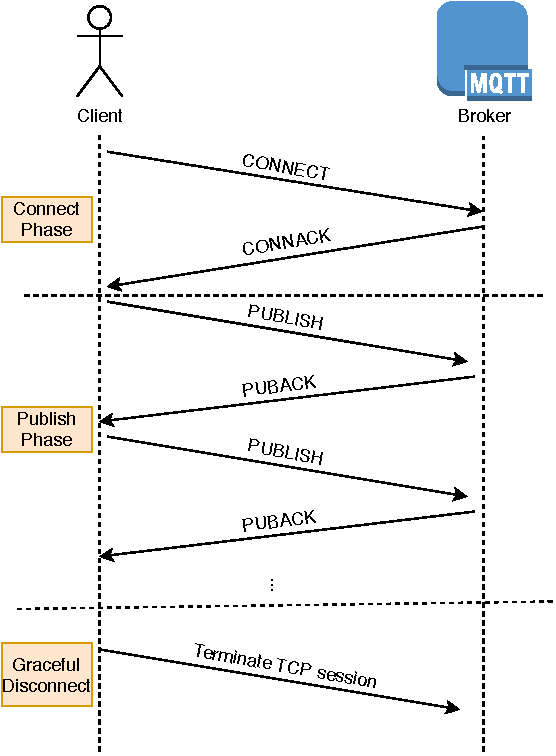
\includegraphics[width=0.6\textwidth]{mqtt_publish}
    \caption{Publishing flow with MQTT}
    \label{fig:mqtt_publish}
\end{figure}


\subsubsection{\textbf{Subscribing}}

Subscribing flow is quite similar to Publishing, with some minor differences. Following figure \ref{fig:mqtt_subscribe}, first and foremost a connection needs to be established by instating standard TCP/TLS session and then sending CONNECT packet. The contents follow the same standard, i.e. containing information such as Client ID or even optional parameters in a form of ``key: value'' (particularly useful for this project).

\begin{figure}[ht]
    \centering
    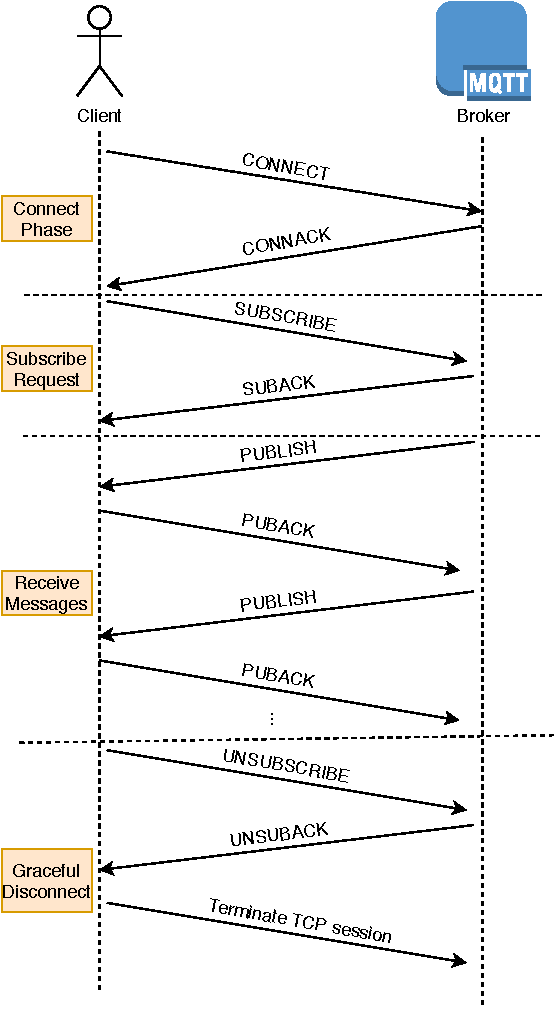
\includegraphics[width=0.6\textwidth]{mqtt_subscribe}
    \caption{Subscribing flow with MQTT}
    \label{fig:mqtt_subscribe}
\end{figure}

After successful connection, Client can proceed to send request for subscription. Similar with PUBLISH packet, client specifies type of the packet in the variable header and then requested topic for subscription in the payload. The extra element is the QOS flag - Quality of Service. MQTT has 3 levels of QOS:
\begin{enumerate}
  \item 0 - No response to PUBLISH messages
  \item 1 - PUBLISH messages will be followed by PUBACK
  \item 2 - More granular control over PUBLISH, with extra packets such as PUBREC (Publish Received), PUBREL (Publish Release) and PUBCOMP (Publish Complete).
\end{enumerate}

Once the SUBSCRIBE message has been processed and approved by the broker, it will issue SUBACK message and remain connect to the client. From this point, any message that is published on the topic specified in SUBSCRIBE packet will be published (as PUBLISH packet) to every client currently subscribed to it. Of course, depending on requested QOS, the broker might then await for PUBACK message (or even issue extra messages such as PUBREC, PUBREL, PUBCOM). The diagram demonstrates a simple exchange with QOS set to 1. 

\begin{table}[h]
\centering
\begin{tabular}{lllllllllllllll}
\cline{1-14}
\multicolumn{1}{|l|}{82} & \multicolumn{1}{l|}{0C} & \multicolumn{1}{l|}{00} & \multicolumn{1}{l|}{01} & \multicolumn{1}{l|}{00} & \multicolumn{1}{l|}{07} & \multicolumn{1}{l|}{F} & \multicolumn{1}{l|}{L} & \multicolumn{1}{l|}{Y} & \multicolumn{1}{l|}{T} & \multicolumn{1}{l|}{R} & \multicolumn{1}{l|}{A} & \multicolumn{1}{l|}{P} & \multicolumn{1}{l|}{00} &  \\ \cline{1-14}
1                        & 2                       & 3                       & 4                       & 5                       & 6                       & 7                      & 8                      & 9                      & 10                     & 11                     & 12                     & 13                     & 14                      &  \\
                         &                         &                         &                         &                         &                         &                        &                        &                        &                        &                        &                        &                        &                         &  \\
                         &                         &                         &                         &                         &                         &                        &                        &                        &                        &                        &                        &                        &                         & 
\end{tabular}
\caption{Example SUBSCRIBE to topic FlyTrap packet}
\label{tab:sub_packet}
\end{table}

To close off MQTT, I also wanted to overview an example packet and dissect it byte by byte to demonstrate exactly what kind of information is included - this can be seen in table \ref{tab:sub_packet}
\begin{enumerate}
  \item [1] Control field, specifies type of the message (CONNECT, SUBSCRIBE etc.)
  \item [2] Remaining length of the message. Can be expanded to 2 bytes.
  \item [3-4] Packet ID
  \item [5-6] Payload length
  \item [7-13] Payload. Corresponding hex encoding of characters, replaced with actual characters for clarity
  \item [14] Requested QOS
\end{enumerate}


\section{Related Work}
This section will talk about other scientific papers which had similar goal in mind, by combining  blockchain technologies with IoT or even MQTT brokers.

